
% Bug: automatically loads natbib with name options, cannot be
% overridden, `Elsevier LaTeX' style produces error messages

\documentclass[review]{elsarticle}
%\documentclass{elsarticle}

\usepackage{hyperref}
\usepackage{lineno,hyperref} \modulolinenumbers[5]
\usepackage{graphicx}
\usepackage{mathtools}
\usepackage{units}
\usepackage{physics} % normal derivative v=dv{x}{t},
                     % partial derivative pdv{V(x,t)}{t}
                     % n'th normal derivative a=dv[2]{x}{t}


\usepackage{color}
\providecommand{\red}[1]{\textcolor{red}{#1}}
\providecommand{\blue}[1]{\textcolor{blue}{#1}}
\definecolor{green}{rgb}{0,0.7,0}
\providecommand{\green}[1]{\textcolor{green}{#1}}

% local macros

\providecommand{\martin}[1]{\red{#1}} %literal, Preprint
\providecommand{\martinc}[1]{\green{[#1]}} %comment, Preprint
%\providecommand{\martin}[1]{#1}                  %fuer Veroeffentlichung
%\providecommand{\martinc}[1]{#1}                  %fuer Veroeffentlichung

\providecommand{\sup}[1]{^{\mathrm{#1}}}  % upright superscript
\providecommand{\sub}[1]{_{\mathrm{#1}}}  % upright subscript $b\sub{comf}$
                                        % symbolic subscripts without:
                                        % $\epsilon_t$
\providecommand{\3}{{\ss}}

\journal{Transportation Research Part C}

%%%%%%%%%%%%%%%%%%%%%%%
%% Elsevier bibliography styles
%%%%%%%%%%%%%%%%%%%%%%%
%% To change the style, put a % in front of the second line of the current style and
%% remove the % from the second line of the style you would like to use.
%%%%%%%%%%%%%%%%%%%%%%%

%% Numbered
\bibliographystyle{model1-num-names}

%% Numbered without titles
%\bibliographystyle{model1a-num-names}
 
%% Harvard
%\bibliographystyle{model2-names.bst}\biboptions{authoryear}

%% Vancouver numbered
%\usepackage{numcompress}\bibliographystyle{model3-num-names}

%% Vancouver name/year
%\usepackage{numcompress}\bibliographystyle{model4-names}\biboptions{authoryear}

%% APA style
%\bibliographystyle{model5-names}\biboptions{authoryear}

%% AMA style
%\usepackage{numcompress}\bibliographystyle{model6-num-names}

%% `Elsevier LaTeX' style
% \bibliographystyle{elsarticle-num}
%%%%%%%%%%%%%%%%%%%%%%%

\begin{document}

\begin{frontmatter}

\title{Formulation and validation of a car-following model based on deep
  reinforcement learning}

%% Group authors per affiliation:
%\author{Fabian Hart\fnref{myfootnote}}
%\address{TU Dresden}
%\fntext[myfootnote]{Comment.}

%% or include affiliations in footnotes:
\author[firstAddress]{Fabian Hart}
\author[firstAddress,secondAddress]{Ostap Okhrin}
\author[firstAddress,secondAddress]{Martin Treiber\corref{corrAuthor}}
\cortext[corrAuthor]{Corresponding author}
\ead{Martin.treiber@tu-dresden.de}
\ead[url]{www.mtreiber.de}

\address[firstAddress]{TU Dresden}
\address[secondAddress]{Possible second address}




\begin{abstract}
To be written at the end
\end{abstract}

\begin{keyword}
reinforcement learning \sep car-following model \sep stochastic
processes \sep string stability \sep validation \sep trajectory data 
\end{keyword}

\end{frontmatter}

%\linenumbers

\section{Introduction}

Autonomous driving technologies are seen as promising solutions to improve road safety, where human errors account for 94\% of the total accidents \cite{vehicleCrashSurvey2015}. Moreover congestion, energy consumption and emissions are intended to be reduced. 
But autonomous driving is a challenging task since the transportation traffic can be dynamic and unpredictable.
On the way to fully autonomous driving, Advanced Driver Assistance Systems
(ADAS) has been developed to solve tasks like lane-keeping, lane-changing, car-following, emergency braking, etc.
Since Deep Learning methods has been demonstrated to surpass humans in certain domains, they are also adopted in the area of autonomous driving.
Especially Deep Reinforcement Learning (DRL), which combines the power of Deep Learning in tackling large, complicated problems with Reinforcement Learning, has shown its potential in a broad variety of autonomous driving tasks. 
In \cite{OnRampMerge2018} and \cite{OnRampMerge2020}, DRL is used to guide an autonomous vehicle safely from on-ramp to freeway. In \cite{intersection1}, \cite{intersection3} and \cite{intersection2}, DRL methods are used to manage traffic of autonomous vehicles at intersections, optimizing safety and efficiency.
In \cite{LangeChange1}, DRL is used to solve lane change maneuvers.

A further task in autonomous driving is to model the vehicle behavior under car following scenarios, where suitable accelerations has to computed in order to achieve a safe and comfortable driving. Approaches to solve this task are classical car-following models, such as the Intelligent Driver Model \cite{Opus} or stochastic car-following models, such as in \cite{Treiber2018stochIDM_TRB}. Furthermore data-driven approaches use Machine Learning methods to train a car-following model based on experimental car-follower data, such as in \cite{Chong2011SimulationOD} or \cite{ZHOU2017245}. Downside of this approach is that the model tries to emulate human driver behavior which still can be suboptimal.

To overcome this issue, DRL methods train non-human car-following models that can optimize metrics such as safety, efficiency and comfort. 
One approach is to train on scenarios, where the leading vehicle trajectory, used for training, is based on experimental data, such as in \cite{SafeEfficientAndComfortable} or \cite{HumanLikeAutonomouCF}. Similar approaches suggest a standardized driving cycle, which functions as leading vehicle trajectory, such as \cite{ComparisonRLvsMPC} or \cite{CFelectricVehicle}, which uses the New European Driving Cycle.
A disadvantage coming along with these approaches is, that for scenarios, which are not in the scope of the training data, the performance decreases, indicating inadequate machine learning generalization \cite{ComparisonRLvsMPC}. 

Another issue of car-following models is string-stability. There are several studies focusing on dampening traffic oscillations by using a sequence of trained vehicles, such as \cite{qu2020jointly}, \cite{DissipatingStopAndGoWaves} and \cite{DampenStopAndGoTraffic}.

All the mentioned DRL car-following models have three disadvantages in common: At first the acceleration range is limited in a way, that full-brakes are not considered. This results in models that are just designed for non-safety-critical scenarios. Second these models just consider car-following scenarios, while free driving or the transition between both is not reflected in the reward function. Third the trained models have just been validated on data that is similar to the training data set, so that the generalization capabilities cannot be proved. 

This motivated us to design a model, which overcomes these issues.
To our knowledge, no RL based car-following model has been proposed which has the following features combined:


\begin{itemize}
	\item  The proposed model considers free driving, car-following, as well as the transition between both in a way, that approaching of the leading vehicle is smooth and comfortable.
	\item The proposed model has a wider range of possible accelerations, which leads to a collision-free behavior also in safety-critical situations such as full-braking of the leader.
	\item The proposed model is trained on leading trajectories, based on an AR(1)-process, e. g. \cite{HonerkampEngl}, the parameters reflecting kinematics of real drivers. This leads to high generalization capabilities and a model usage in a broader variety of traffic scenarios. 
	\item Different driver characteristics can be modeled by adjusting the parameters of the reward function.
	\item The proposed model shows string-stability.
	
\end{itemize}

Another feature of this work is a thorough validation of the above mentioned properties in scenarios based on both synthetic and naturalistic trajectory data, bringing the model to its limits. 
In all cases, the model proved to be accident free and string stable.
In a further experiment the proposed model is compared to an Intelligent Driver Model, calibrated on the same data. The results indicate a better performance of the proposed model.


[short textual enumeration of the sections to come]

\section{Model specification}
The \martin{following vehicle} \martinc{only named things are written
    in uppercase; special concepts/definitions such as Reinforcement Learning
    can be written both upper and lowercase; abbreviation always
    uppercase (RL); the
    ``reward function'' is generic, hence lowercase} is controlled by a Reinforcement
Learning (RL) agent. By interaction with an environment, the RL agent
optimizes a sequential decision making problem. At each time step
$t$,\martinc{always comma before the main clause starts} the agent
observes an environment state $s_t$ and, based on that state, selects
an action $a_t$. After conducting action $a_t$, the RL agent receives
a reward $r(a_t,s_t)$. The agent aims to learn an optimal state-action
mapping policy $\pi$ that maximizes the expected accumulated
discounted reward. \martinc{Du musst zwischen der Summe $R_t$  und den
  Termen $r_t$ unterscheiden. W\"are links $r_t$, w\"are dies ein
  Gleichungssystem mit den L\"osungen $\{r_t=0 \forall t \} $ oder
  $\{r_t\to\infty \forall t \} $. Diese wichtige Formel verdient eine
  eigene Nummer.}
\begin{equation}
\label{Rt}
R_{t}=\sum_{k=0}^{\infty} \gamma^{k} r_{t+k},
\end{equation}
 where $\gamma = (0,1]$ denotes the discount factor and 
$\gamma^k r_{t+k}$ the expected contribution $k$ time steps ahead. The crucial elements
of the RL-based \martinc{use your abbreviation} control strategy are described
in detail as follows:

\subsection{Action space}
\label{actionSpace}
In this study, the acceleration of the following vehicle is considered
as the action of the RL agent. To enable comfortable driving and
\martin{allow for a maximum braking deceleration} in safety-critical
situations, the acceleration \martin{is a continuous variable in the
  range} between $a_{\rm min} = \unit[-9]{m/s^2}$ and 
$a_{\rm max} =\unit[2]{m/s^2}$.\martinc{In contrast to variables or symbolic
    constants which are set in italic, units are set in roman
    (upright) font. If super- or subscripts are variables, they are
    set italic. If they are abbreviations (e.g., min, max) they are set
    upright. Multi-letter standard function names such as $\sin$,
    $\tan$, $\cosh$ or $\exp$ are written upright (use
    \texttt{\$\textbackslash sin\$} etc)}


\subsection{State space}
The state space defines the observations \martin{that} the following
vehicle can receive from the environment. To compute an optimal
acceleration, the following vehicle observes its own acceleration $a$,
its own \martin{speed}\martinc{velocity=vector, speed=abs(velocity)=scalar}
$v$, the \martin{relative speed $\Delta v=v_l-v$ where $v_l$ denotes
  the speed of the leading vehicle} \martinc{crucial since both definitions
    $v_l-v$ or $v-v_l$ are common} and the \martin{(bumper-to-bumper)
  gap $s$ to the leader} \martinc{again, some use the space headway (including
    the leading vehicle length), and some the gap}. These
observations are normalized to the range $[-1,1]$. \martinc{How? If it
    is just linear translation and scaling, you need min and max
    values of the state variables. How to determine them?}


\subsection{Reward Function}
\label{rewardFunction}
The goal of the RL strategy is to reduce the crash risk, while
maintaining comfortable driving in non-safety-critical situations
\martin{and minimizing the travel time} \martinc{without that, creeping which
    is safe and comfortable would be the optimum strategy}. The
\martin{r}eward function includes a set of parameters that can be
adjusted to realize different \martin{driving} styles. $v_{\rm des}$
is the desired speed that should not be exceeded. $a_{\rm min}$ and
$a_{\rm max}$ are the minimum and maximum possible accelerations, as
described in Section \ref{actionSpace}. All parameters are described
in Table \ref{tab:agentParameters}.
\martin{Ich habe die simultan
  verwendeten bezeichnungen $T$ und $T\sub{opt}$ in $T$
  umbenannt.} 

\begin{table}
\caption{RL agent parameters and default values \martinc{check the weights!}} 
\label{tab:agentParameters} 
\begin{center}
\begin{tabular}{ p{0.12\textwidth}| p{0.65\textwidth}| p{0.1\textwidth}}
	Parameter & Description & Value \\ \hline
	$a_{\rm min}$ & Minimum acceleration & $\unit[-9]{m/s^2}$ \\  
	$a_{\rm max}$ & Maximum acceleration & $\unit[2]{m/s^2}$ \\  
	$b_{\rm comf}$ & Comfortable deceleration & $\unit[-2]{m/s^2}$ \\  
	$v_{\rm des}$ & Desired speed & $\unit[16.6]{ m/s}$ \\  		
	$T$ & Desired time gap to the leading vehicle & $\unit[1.5]{s}$ \\
	$s_{\rm min}$ & Desired minimum space gap & $\unit[2]{m}$ \\
	$T_{\rm var}$ & \martin{Time gap parameter (cf Eq. \eqref{eq:r12})} & $\unit[0.7]{s}$ \\
	$T_{\rm lim}$ & Upper time gap limit for zero reward (see
        Eq. \eqref{eq:r1}) & $\unit[15]{s}$ \\
  $w_1$ & \martin{relative weight for keeping the desired gap} & 0.6\\
  $w_2$ & \martin{relative weight for driving safely} & 1.1\\
  $w_3$ & \martin{relative weight for driving comfortably} & 0.001\\
\end{tabular}
\end{center}
\end{table}


\martinc{first describe the element shortly, then come with
    the formulas}
The reward function contribution at time step $t$ consists of four factors. \martin{not parts; the
    parts are the weighted factors, see~\eqref{reward}}
The first part aims \martin{to not fall below} \martinc{above is OK: free flow} a reasonable
distance to the leading vehicle. 

\martinc{The standard normal distribution has the symbol $\Phi(.)$ and
    its density $\phi(.)$ or $\varphi(.)$; I prefer $\varphi$ since, then,
    the optical difference to the CDF $\Phi$ is greater}
\martinc{Use \texttt{\textbackslash left( ... \textbackslash right)}
    to make ``bigger'' parentheses, brackets, braces around fractions
    or super- and subscript quantities}

\martinc{Warum nicht einfach $r_1=1-((s-s\sub{opt})/s\sub{opt})^2$
  f\"ur $s\le s\sub{opt}$ und $r_1=1$ sonst? Das erspart 2
  Parameter, 2 Gleichungen und die komischen Ad-Hoc Zahlen 0.5 und 2}
\begin{equation}
\label{eq:r1}
r_1  = 
\begin{cases}
\frac{\varphi((s-s\sub{opt})/s\sub{var})}{\varphi(0)},
  & \text{if } s < s^*\\
\frac{\varphi((s-s\sub{opt})/s\sub{var})}{\varphi(0)}
 \left(1-\frac{s-s^*}{s\sub{lim} - s^*}\right)  & \text{otherwise}
\end{cases}
\end{equation}
with
\begin{equation}
\label{eq:r11}
s\sub{opt} = vT + s\sub{min},
\end{equation}
\begin{equation}
\label{eq:r12}
s\sub{var} = vT\sub{var} + 0.5s\sub{min},
\end{equation}
\begin{equation}
\label{eq:r13}
s\sub{lim} = vT\sub{lim} + 2s\sub{min},
\end{equation}
%
and $\varphi(x)$ describing the standard-normal probability density
function. \martinc{No empty line if no new paragraph; otherwise, you get an
  indent that looks strange] [$s^*$ is not defined}.

Figure \ref{fig:RewardFunc1} illustrates the reward function for
$r_1$, containing the parameter $s\sub{opt}$, $s^*$ and $s_{\rm
  lim}$. \martinc{Schaut man auf die Grafik, erweckt dies den
    Eindruck, dass $s^*$ von $s\sub{lim}$ und $s\sub{opt}$ abh\"angt,
    genau so, dass die Funktion differenzierbar ist. Warum nicht
    $s\sub{lim}\to \infty$ setzen? Das bedeutet lediglich, dass
    dieser Teil der Reward-Funktion indifferent gegen sehr gro\3e
    Abst\"ande ist (``es ist egal, ob der Abstand $s\sub{opt}$ oder
    $\infty$ ist, Hauptsache, er ist nicht kleiner''). Falls
    $v<v\sub{des}$ ist, wird sich der realisierte Abstand dennoch auf
    $s\sub{opt}$ einstellen. Au\3erdem spricht der n\"achste Teil der
    Reward-Funktion ggf auch auf gr\"o\3ere Abst\"ande an} 
The reward function is designed in a way, that for high speeds $v$
of the following vehicle the time gap between following and leading
vehicle tends to $T$, while for low speeds the distance
between both tends to $s\sub{min}$. Different values of $T$
result in different driving styles in a way that, for \martin{lower} values of
$T$ \martin{and $s\sub{min}$,} the \martin{driver follows
  more closely the leading vehicle} resulting in a more aggressive
driving style. The results for different values of $T$ can
be found in Section \ref{sec:differentT}. Different functions for $ s
> s^*$ has been applied, but the best results regarding a smooth and
comfortable approaching of the following vehicle has been reached with
a linear function. Also, a high value of $T\sub{lim}$ results in an
early deceleration and comfortable approaching. \martinc{Daf\"ur
  sollte eigentlich ein Anteil $\propto (v-v_l)/s$ zust\"andig sein;
  bis jetzt kommt die ``relative speed'' nur quadratisch vor} 

The second factor of the reward function addresses the \martin{driver's
  response} in safety-critical situations \martin{by comparing the
  kinematically needed deceleration $(\Delta v)^2/(2s)$ (assuming an
  unchanged speed of the leader) with the
  comfortable deceleration $b\sub{comf}$,}

\begin{figure}
	\centering
	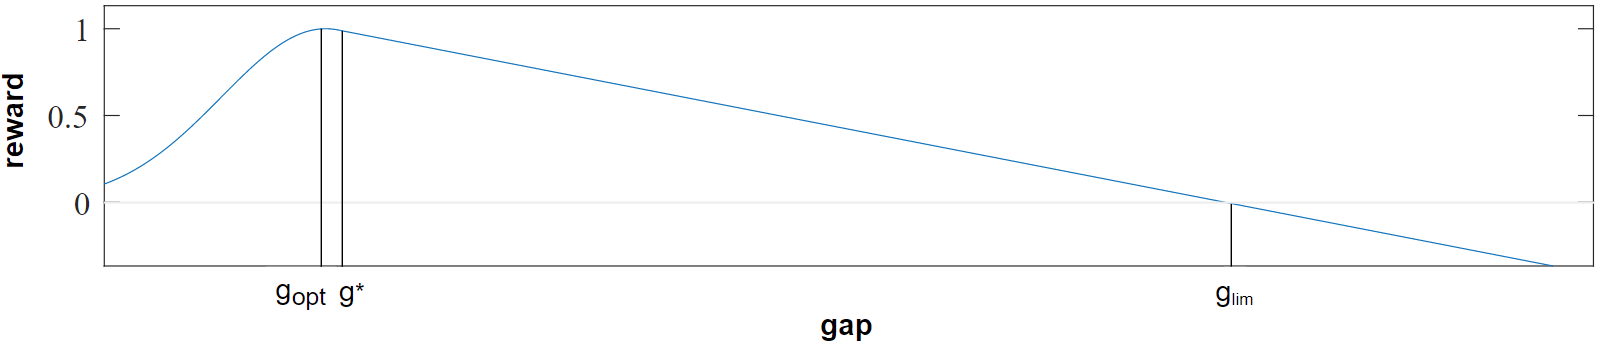
\includegraphics[width=12cm]{images/RewardFunc1}
	\caption{Factor 1 of the reward function maximizing the reward
          for car following with time gap $T$} 
	\label{fig:RewardFunc1}
\end{figure}


\begin{equation}
\label{r2}
r_2 = 
\begin{cases}
\tanh\left(\frac{b_{kin}-b\sub{comf}}{b\sub{min}}\right),& \text{if } b_{kin}>b\sub{comf}\\
0,              & \text{otherwise}
\end{cases}
\end{equation}

with
\begin{equation}
b_{kin} = \frac{\Delta v^2}{s}
\end{equation}
\martinc{Ich habe nun nur noch ``instruktive'' \"Anderungen markiert}
The argument of the tanh function with  the
  maximum possible deceleration ($\approx 1 g$ on dry roads) gives a
  non-dimensional measure for the seriousness of the critical situation
  with values 
  near or above 1 indicating an imminent crash. \martinc{$b\sub{max}$
    or $-a\sub{min}$}. Notice that the case distinction in
~\eqref{r2}  ensures that
this term is not activated in non-critical situations as illustrated in Fig.~\ref{fig:xy}. \martinc{Das
    f\"uhrt aber evtl zu einer ``Stotterbremse'' beinm Ann\"ahern an
    stehende Fahrzeuge, da dann $r_1$ in der Regel nicht gen\"ugend
    Bremskraft entwickelt}

The third factor of the reward function aims to reduce the jerk in
order to achieve comfortable driving, \martinc{\textbackslash dv from
  the physics package; notice the upright 'd's}
\martinc{$r_3$ muss einheitenlos sein, sonst vergleicht man in
  \eqref{rt} \"Apfel mit Birnen! Check, ob das Gewicht $w_3$ noch
  stimmt (Tabelle)}
\begin{equation}
r_3 = -\left(\frac{1}{b\sub{comf}} \ \dv{a}{t}\right)^2.
\end{equation}
%
Since building up a comfortable value of acceleration or deceleration
from zero in one second is at the limit of comfortable jerks, $r_3$
values above unity tend to feel uncomfortable. 

 The fourth factor of the reward function penalizes the RL agent, if
 the current speed $v$ is above the desired speed $v\sub{des}$,
 \martinc{Einheitenlos! Schon wegen des Vergleichs mit 1, aber auch,
   um keine \"Apfel und Birnen in~\eqref{rt} zu vergleichen!}
\begin{equation}
r_4 =  
\begin{cases} 
 -\min\left[1,\left(\frac{v - v\sub{des}}{v\sub{des}}\right)^2\right], & \text{if } v>v\sub{des}\\
0, & \text{otherwise.}
\end{cases}             
\end{equation}
%
\martin{The contribution of the final reward function~\eqref{Rt}  at simulation time step $t$ is the weighted
sum of these factors according to}\martinc{Die Gewichte $w_1$
  ... $w_3$ sind wichtige Modellparameter. Ich habe sie deshalb als
  solche benannt und in Table \ref{tab:agentParameters} eingef\"uhrt}
\begin{equation}
\label{rt}
%r_t = 0.6r_1 + 1.1r_2 + 0.001 r_3 + r_4,
r_t = w_1r_1 + w_2r_2+w_3r_3 + r_4,
\end{equation}
\martin{where all the factors are evaluated at time step $t$. The weights (cf.
Table~\ref{tab:agentParameters})} have been found experimentally and
can be optimized in future studies. \martin{Notice that the weights are
relative weights related to the incentive of driving at the desired
speed.}


\subsection{\label{RL-algorithm}RL algorithm}
In various similar control problems, the Deep Deterministic Policy
Gradient (DDPG) Algorithm has been used and proven to perform well on
tasks with a continuous action and state space, such as in
\cite{SafeEfficientAndComfortable}, \cite{ComparisonRLvsMPC} or
\cite{HumanLikeAutonomouCF}. The original work can be found in
\cite{DDPG}. In order to reduce the variance of policy gradients and
increase learning speed, DDPG is an actor-critic method. \martinc{Was
  ist eine ``policy'' bzw ein ``policy gradient'' in diesem Kontext? TRB und TRC sind nicht spezialisiert
  auf Deep Learning Methods, deshalb ist ein Satz Erkl\"arung n\"otig} The actor determines the action, while the critic judges about the quality of the action and how the policy should be adjusted. In this study, both networks are feed-forward neural networks with two layers of hidden neurons and 32 neurons each hidden layer. All DDPG parameters are presented in Table \ref{tab:DDPGparameters}.

\begin{table}
	\caption{DDPG parameter values} 
	\label{tab:DDPGparameters} 
	\begin{center}
		\begin{tabular}{ p{0.4\textwidth} p{0.2\textwidth} }
			Parameter & Value \\ \hline
			Learning rate & 0.001 \\ 
			Reward discount factor & 0.95 \\ 
			Experience buffer length & 100000 \\ 
			Mini batch size & 32 \\ 			
			Gaussian noise mean & 0.15 \\ 
			Gaussian noise variance & 0.2 \\ 
			Gaussian noise variance decay  & 1e-5 \\ 
			Number of hidden layers & 2\\
			Neurons per hidden layer & 32\\
			

		\end{tabular}
	\end{center}
\end{table}


\subsection{Reward Function}
\martinc{Die wurden bereits in Abschnitt~\ref{rewardFunction}
  spezifiziert. Parameter sollten auch dort erkl\"art werden. Wie man
  die reward function in den RL-Algorithmus einbaut, sollte in
  Sec~\ref{RL-algorithm} erkl\"art werden. Insbesondere, wie man die
  eigenen Bewegungen (konstante Beschleunigung?) und die Bewegungen
  des Leaders voraussagt, um $r_{t+k}$ f\"ur die Zukunft ($k$
  Zeitschritte im
  Vorraus) bestimmen zu k\"onnen und wie gro\3 der prediction time
  horizon ist}



\section{Model training}
The training of the model comprises two important components, which
have to be defined in advance: Generation of trajectories for the
leading vehicle and
the specification of a training episode.

\subsection{Generating synthetic trajectories for the leading vehicle}
The leading trajectory is based on an AR(1) process, whose parameters
reflect the kinematics of real leaders. The AR(1) process describes
the speed of the leading vehicle and is defined as \martinc{Habe ich
  pr\"azisiert} 

\begin{equation} \label{eq:AR1}
	v_l(t) = c+\phi v_l(t-1)+ \epsilon_t
\end{equation}
with
\begin{equation}
    E(\epsilon_t) = 0, \ \text{Var}(\epsilon_t) = \sigma, \ 
\text{Cov}(\epsilon_t\epsilon_{t+k})=0 \text{ for }k\neq 0
\end{equation}

After reaching stationarity, this process has 
\begin{equation}
\label{eq:E_AR1}
 \text{the expectation value }E(v_l) = \frac{c}{1-\phi}, 
 \end{equation}
 
 \begin{equation}
 \label{eq:V_AR1}
 \text{the variance }\text{Var}(v_l) = \frac{\sigma^2}{1-\phi^2}, 
 \end{equation}

 \begin{equation}
 \label{eq:ACF_AR1}
\text{the autocorrelation  }\text{ACF}(dt) = \phi^{dt}, 
\end{equation}

 \begin{equation}
 \label{eq:tau_AR1}
\text{and the correlation time  }\tau = -\frac{1}{\ln \phi}, 
\end{equation}
\martinc{multi-letter special functions $\sin, \cos, \tan, \ln, \tanh
  ...$ have latex macros}
with $d$ corresponding to the simulation step size, which is globally
set to \unit[100]{ms}. \martinc{use the \textbackslash unit macro applicable
  in text and math mode. As in the multi-letter math functions, this
  controls the space after it ($>0$, less than a normal text space)} 

To adjust the parameters of the AR(1) process, typical values for real leader trajectories has to be defined: With $v_{l,des}$ as the desired speed for the leader, the mean of the AR(1) process is set to be $v_{l,des}/2$ and the standard deviation is set to be $v_{l,des}$. The acceleration $a\sub{phys}$ corresponds to typical physical leader accelerations. With these values and by using Equation \eqref{eq:E_AR1} - \eqref{eq:tau_AR1}, the parameters of the AR(1) process can be calculated as:

 \begin{equation}
\phi = e^{(\frac{-2da\sub{phys}}{v_{l,des}})},
\end{equation}

 \begin{equation}
c=(1-\phi)\frac{v_{l,des}}{2},
\end{equation}

 \begin{equation}
 \sigma^2=(1-\phi^2)\frac{v_{l,des}^2}{4}.
\end{equation}
The assumed typical values for $v_{l,des}$ and  $a\sub{phys}$ as well as the resulting values of the AR(1) process parameters can be found in Table \ref{tab:AR1Parameters}.

\begin{table}
	\caption{Assumed typical values for leading trajectories and
          the resulting values of the AR(1) process parameters \martin{for an
          update time step of \unit[100]{ms}}} 
	\label{tab:AR1Parameters} 
	\begin{center}
		\begin{tabular}{ p{0.1\textwidth} p{0.1\textwidth} |p{0.1\textwidth} p{0.1\textwidth}  }
			 \multicolumn{2}{c|}{Real trajectory} & \multicolumn{2}{c}{AR(1) process}   \\ \hline
			$v_{l,des}$ &$\unit[15]{m/s}$ &$\phi$ & $0.9933$\\
			$a\sub{phys}$ &$\unit[1]{m/s^2}$ &$c$ & $\unit[0.05]{m/s}$\\
			& & $\sigma^2$ & $\unit[0.75]{m^2/s^2}$
			
		\end{tabular}
	\end{center}
\end{table}

Figure \ref{fig:AR1process} shows an example trajectory of the leading vehicle based on the AR(1) process using the parameters of Table \ref{tab:AR1Parameters}. If the speed exceeds the defined range of $[0, v_{l,des}]$, it is manually set to the range limits.
\begin{figure}
	\centering
	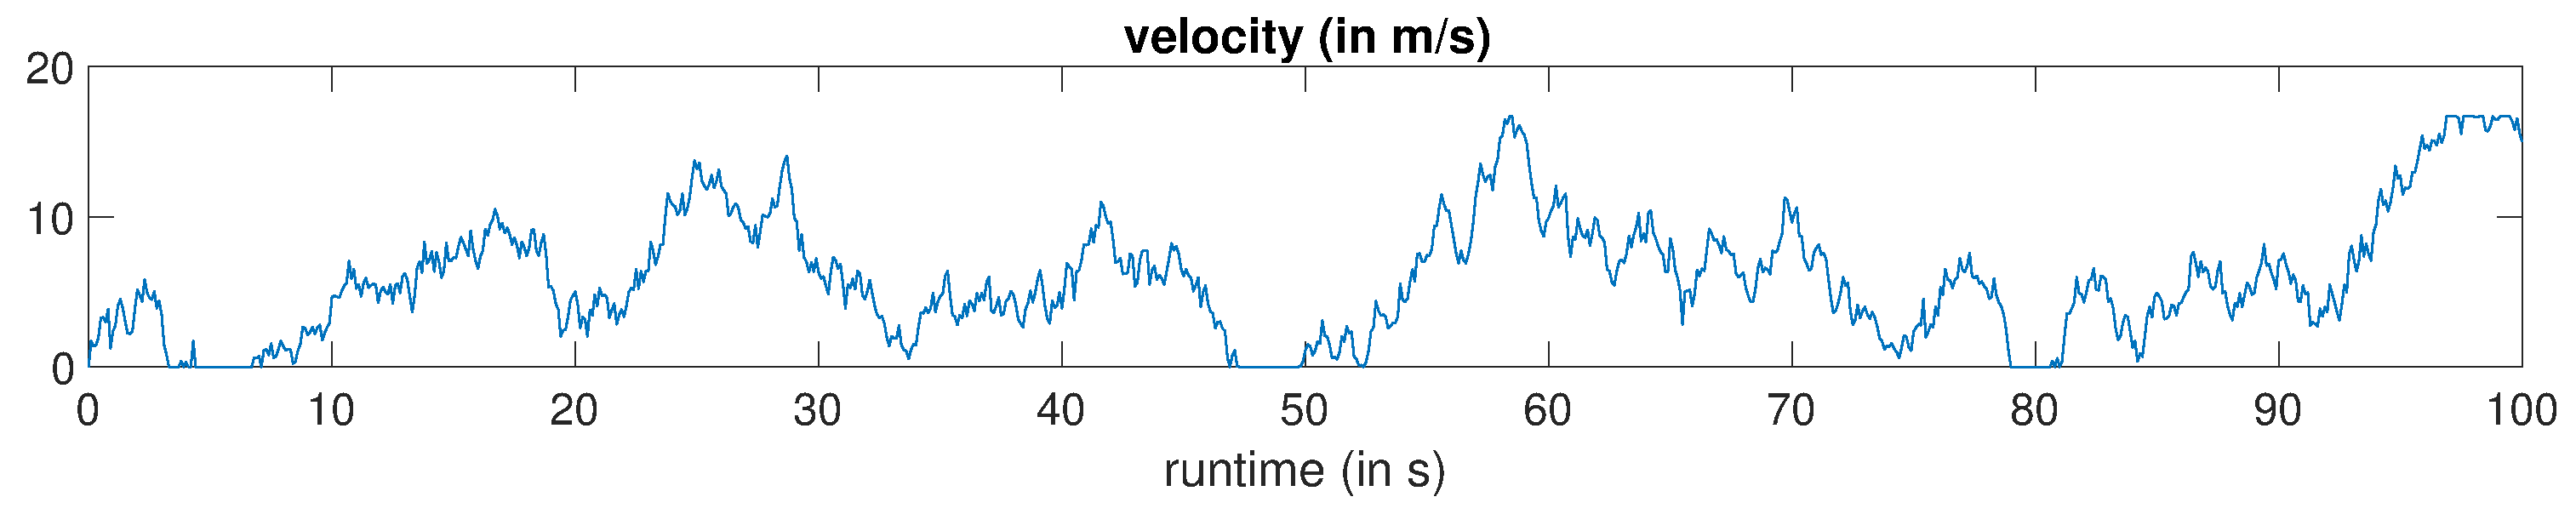
\includegraphics[width=0.95\textwidth]{images/AR1process}
	\caption{Example of a leading trajectory based on the parametrized AR1 process used to train the RL agent}
	\label{fig:AR1process}
\end{figure}


\begin{figure}
	\centering
	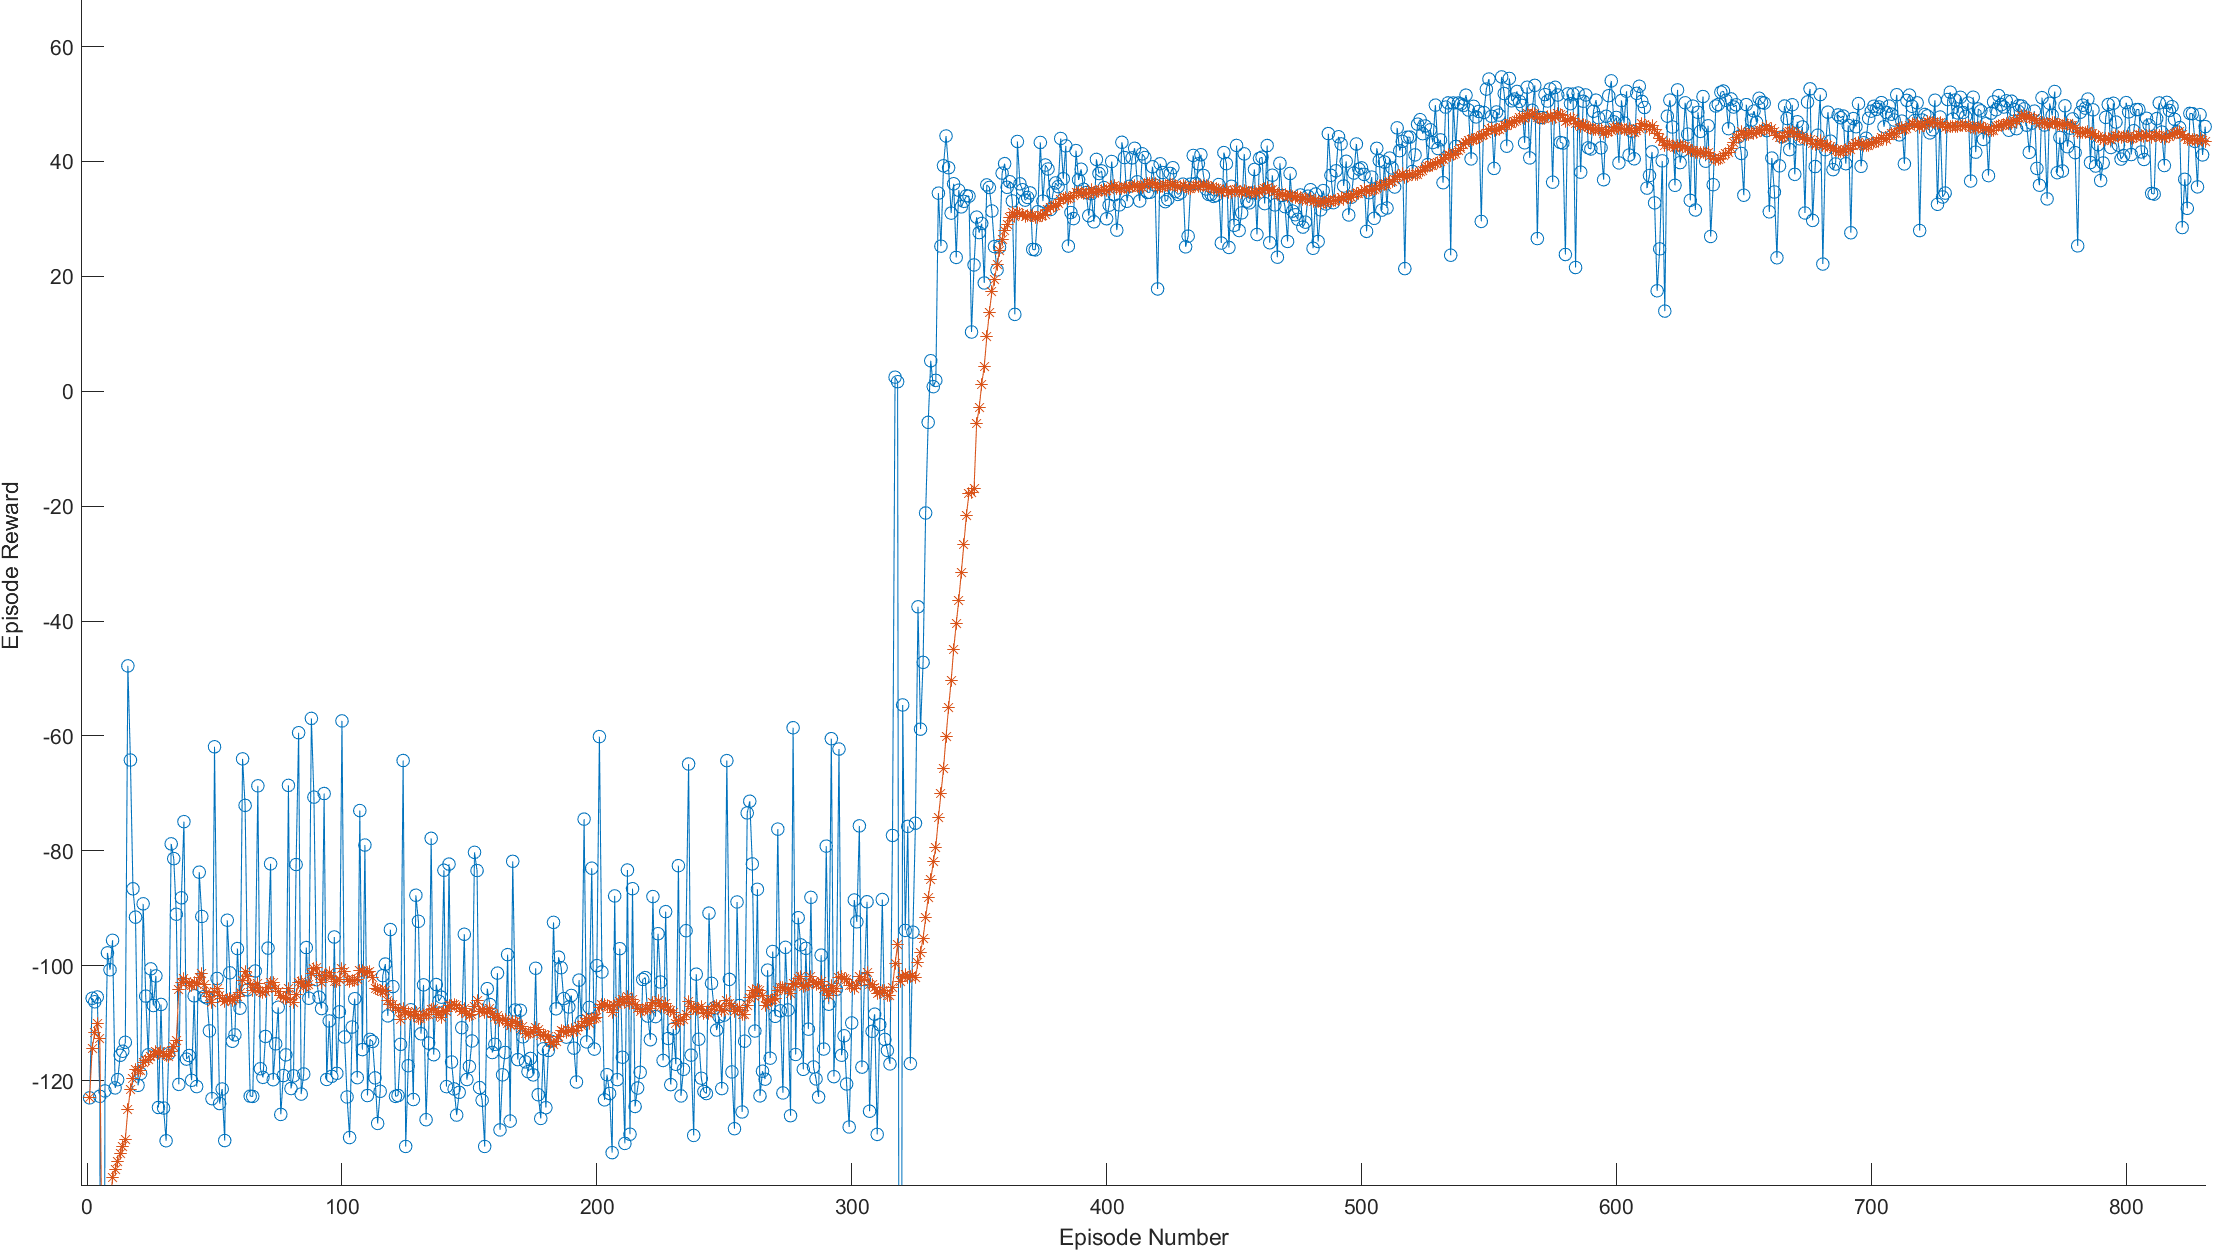
\includegraphics[width=0.95\textwidth]{images/Training}
	\caption{RL training process, one episode contains 500
          steps. Shown are the reward values of the individual
          episodes (blue) and a 50-step asymmetric moving average
          \martinc{Im Gegensatz zum exponential moving average ist der
          normale moving average standardm\"a\3ig symmetrisch,
          enth\"alt also Vergangenheit und Zukunft.}}
	\label{fig:training}
\end{figure}

\subsection{Training episode definition}

To train the RL agent, a training episode has to be defined. One
episode has a simulation time of \unit[50]{s} with a step size of
$d=\unit[100]{ms}$ resulting in an episode length of $500$
steps.\martin{Reine Zahlen (aber nicht das Minus-Zeichen!) sind im Text- und Math-Modus gleich. Ebenso
  wie Einheiten ohne Exponent ben\"otigen positive Zahlen keine Dollars, also 500
  steps oder \unit[50]{s} mit oder ohne \$ OK}   The initial
speeds of \martin{the} following and leading \martin{vehicles are
  randomly}  set in the range $[0,v\sub{des}]$ and $[0,v_{l,des}]$,
respectively. \martinc{``respectively'' kommt immer, mit Komma
  abgetrennt, nach der Aufz\"ahlung, auch bei zwei items} The initial
space gap between both is set to \unit[120]{m}. 

\subsection{Results of the RL training process}

Figure \ref{fig:training} shows an example of the training
process. The red line shows the moving average reward of the last 30
episodes. After approximately 570 episodes\martin{,} the maximum
average reward has been reached. \martin{Once the saturation has been
confirmed at an episode count of 850, the learning
process has been stopped.} \martinc{Das Maximum war
  doch schon bei 570. Warum saturation erst bei 850? Ich habe es so
  umformuliert wie ich denke, dass der Algo l\"auft. \"Ubrigens sollte
  man den Sprung nach etwa 350 Episoden erkl\"aren. Ist das der
  typische Fall? Falls ja, kann es passieren, dass der Algo vorher
  stoppt, da er nicht mehr denkt, dass noch ein Sprung kommt?}

\section{Validation}

The goal is not to minimize some error measure as in usual
calibration/validation but to check if the driving style is safe,
effective, and comfortable. The RL strategy is evaluated with respect to these metrics in different driving scenarios, described in the following.

\subsection{Response to an external leading vehicle speed profile}
The first scenario is designed in order to evaluate the transition between free driving and car-following as well as the follower's behavior in safety-critical situations. 
Figure \ref{fig:manipulatedLeader} shows a driving scenario with an
artificial external profile for the leading vehicle speed. The initial
gap between 
follower and leader is 200 meters, which refers to a free driving
scenario. The follower accelerates with $a\sub{max} = 2m/s^2$ until
the desired speed $v\sub{des} = 16.6m/s$ is reached and approaches
the standing leading vehicle. When the gap between both drops below 90
meters, the follower starts to decelerate with a \martin{maximum
  deceleration of} approximately $b_{\rm
  comf} = \unit[2]{m/s^2}$ (transition between free driving and car-following)
and comes to a standstill with a final gap of approximately 
$s\sub{min} = \unit[2]{m}$. \martin{Afterwards ($t=\unit[27]{s}$),  the leading vehicle accelerates to a speed
that is below the desired speed of the follower before performing a
maximum braking maneuver ($a=\unit[-9]{m/s^2}$) to a full stop ($t=\unit[40]{s}$).} \martinc{Die Beschleunigung
  ist \emph{nicht} random}. \martin{At the time of the start of the
  emergency braking, the follower has nearly reached a steady
  following mode at the desired space gap $s=s_0+v_l T$. While this
  gap makes it impossible to keep the deceleration in the comfortable
  range without a rear-end collision, the follower makes the best of
  the situation by braking smoothly with a maximum deceleration of $-a
  \approx \unit[5]{m/s^2}$.  The transition between different
accelerations happens in a comfortable way reducing the resulting
jerk. Only at the beginning ($t=\unit[39]{s}$) where the situation is
really critical, the jerk $\text{d}a/\text{d}t$ exceeds the comfortable range 
$\pm \unit[1.5]{m/s^3}$. Afterwards, the leader performs a series of
non-critical acceleration and deceleration maneuvers and the follower
tries to follow the leader at the speed dependent desired space gap
$s_0+v_lT$ while 
simultaneously smoothing the leader's speed profile.} 



\begin{figure}
	\centering
	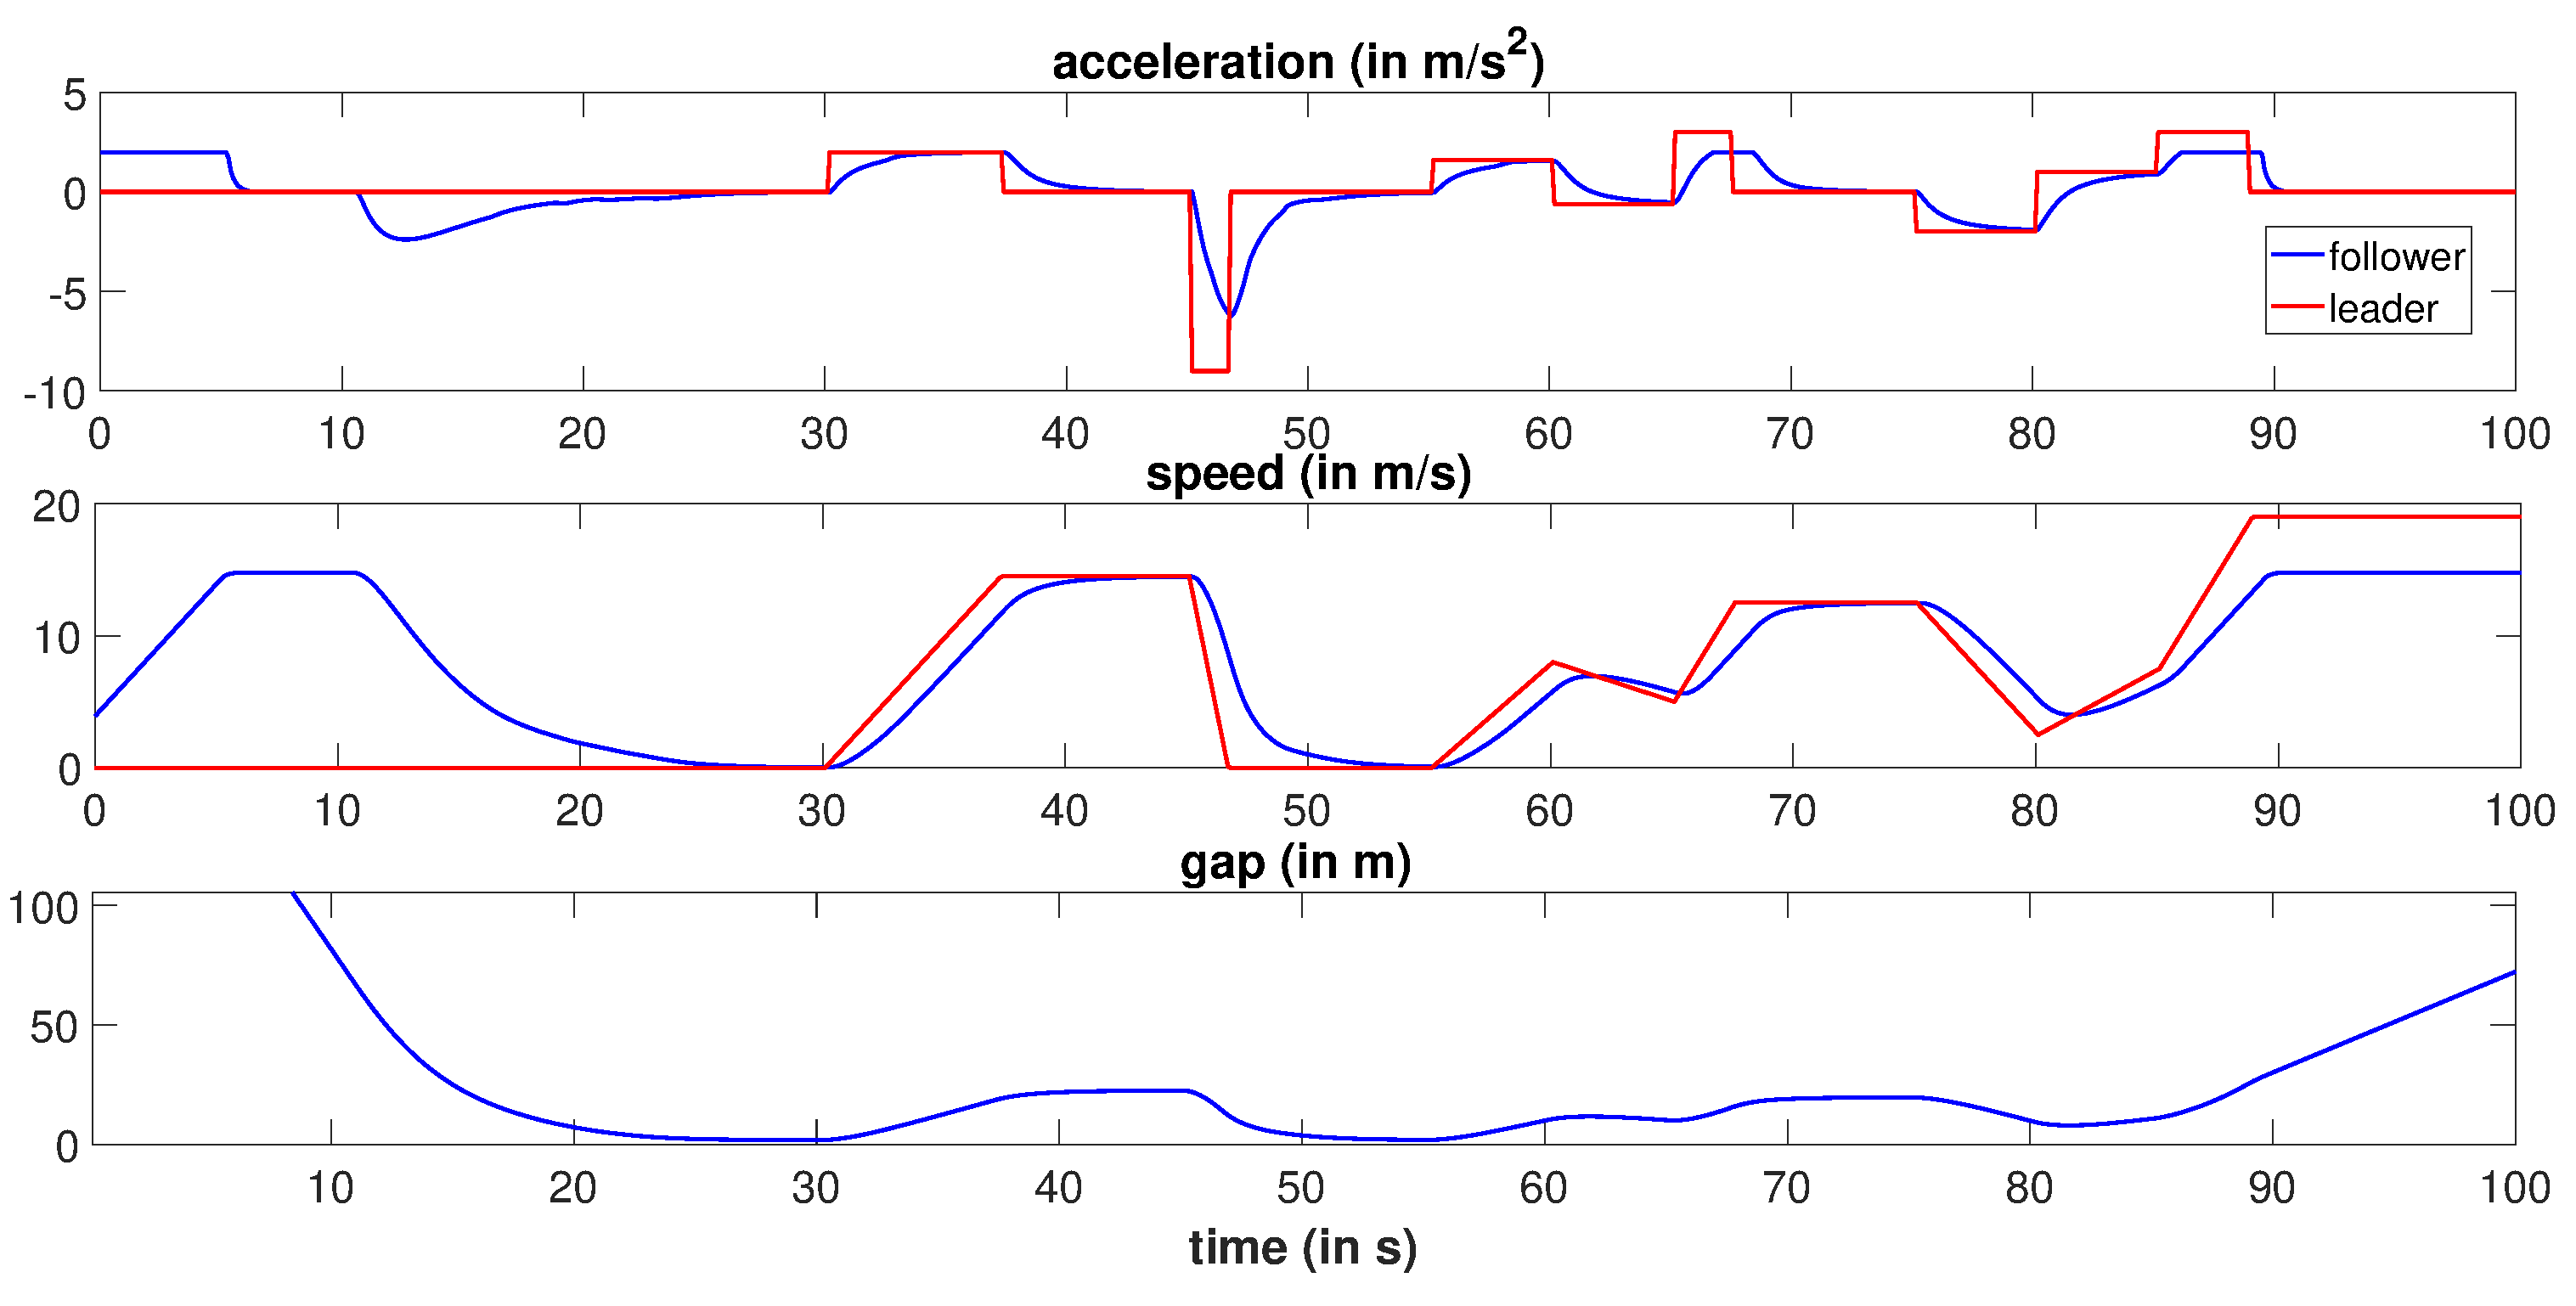
\includegraphics[width=0.95\textwidth]{images/manipulatedLeader.eps}
	\caption{Response to an external leading vehicle speed profile
\martinc{runtime $\to$ time, da sich runtime so nach Computerlaufzeit
  anh\"ort, distance $\to$ gap. Dort sollte man die Skala nur bis
  \unit[50]{m} gehen lassen, da man sonst fast nichts sieht,
  insbesondere nicht, ob $s\sub{des}$ ann\"ahernd eingehalten wird.} }
	\label{fig:manipulatedLeader}
\end{figure}

\begin{figure}
	\centering
	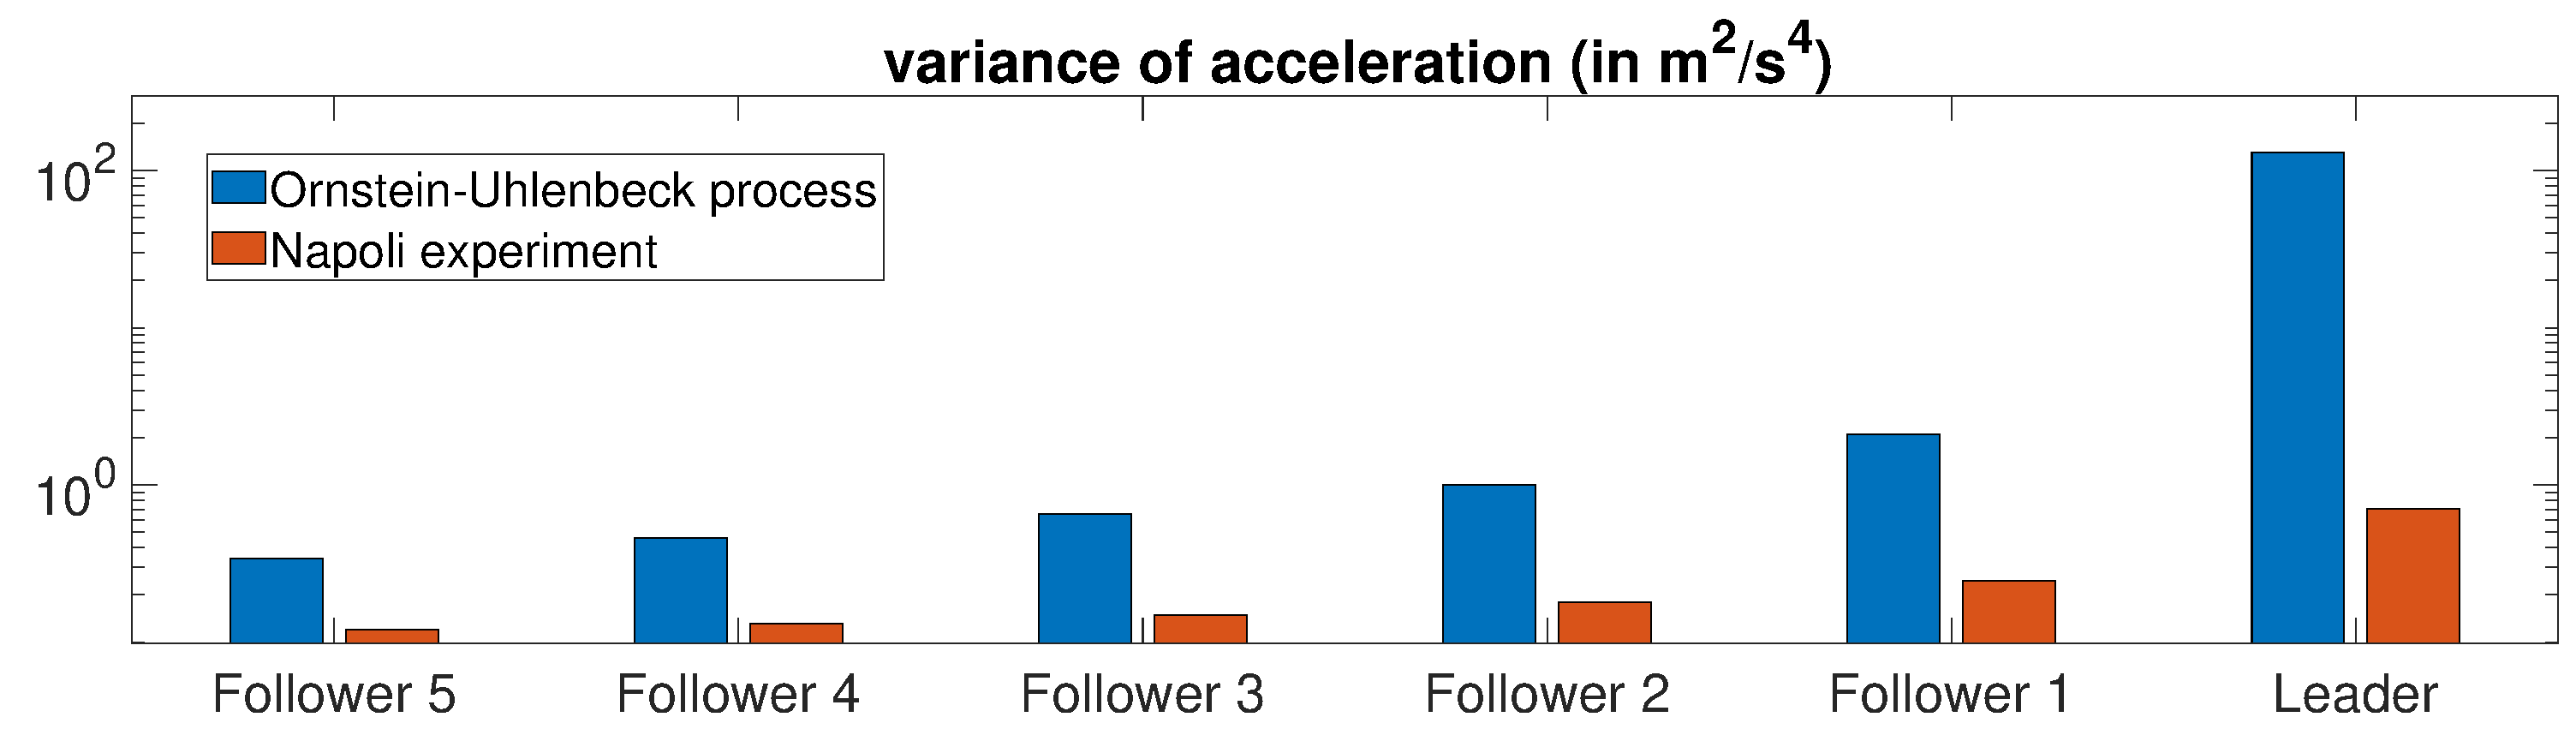
\includegraphics[width=0.95\textwidth]{images/VarAccComp}
	\caption{Comparison of the acceleration variance between
          leader and follower for a leader controlled by AR(1) (blue
          bars) and the leading vehicle of the Napoli experiment
          (red).
\martinc{Die Varianz hat die Einheit $\unit{m^2/s^4}$ (Korrektur in der
Grafik!) In der Tat stimmt der blaue Balken des Leaders, der eine
H\"ohe von $\sigma^2/d^2=\unit[75]{m^2/s^4}$ haben sollte}}
	\label{fig:VarAccComp}
\end{figure}






\subsection{String stability}
\label{sec:stringStability}
The second \martin{validation} scenario, shown in Figure
\ref{fig:AR1Kolonne}, consists of a leader based on the AR(1) process
that is
followed by five vehicles, each controlled by the trained RL
agent. The results show that traffic oscillations can effectively be
dampened with a sequence of trained followers, even if the leader
shows large outliers in acceleration. Figure \ref{fig:VarAccComp}
illustrates the difference of accelerations between leader and the
followers (blue bars). The last follower shows the lowest variance of
acceleration, which demonstrates the ability of the RL agent to
flatten the speed profile, to dampen oscillations and thus to increase
comfort and reduce fuel consumption and emissions.   


\begin{figure}
	\centering
	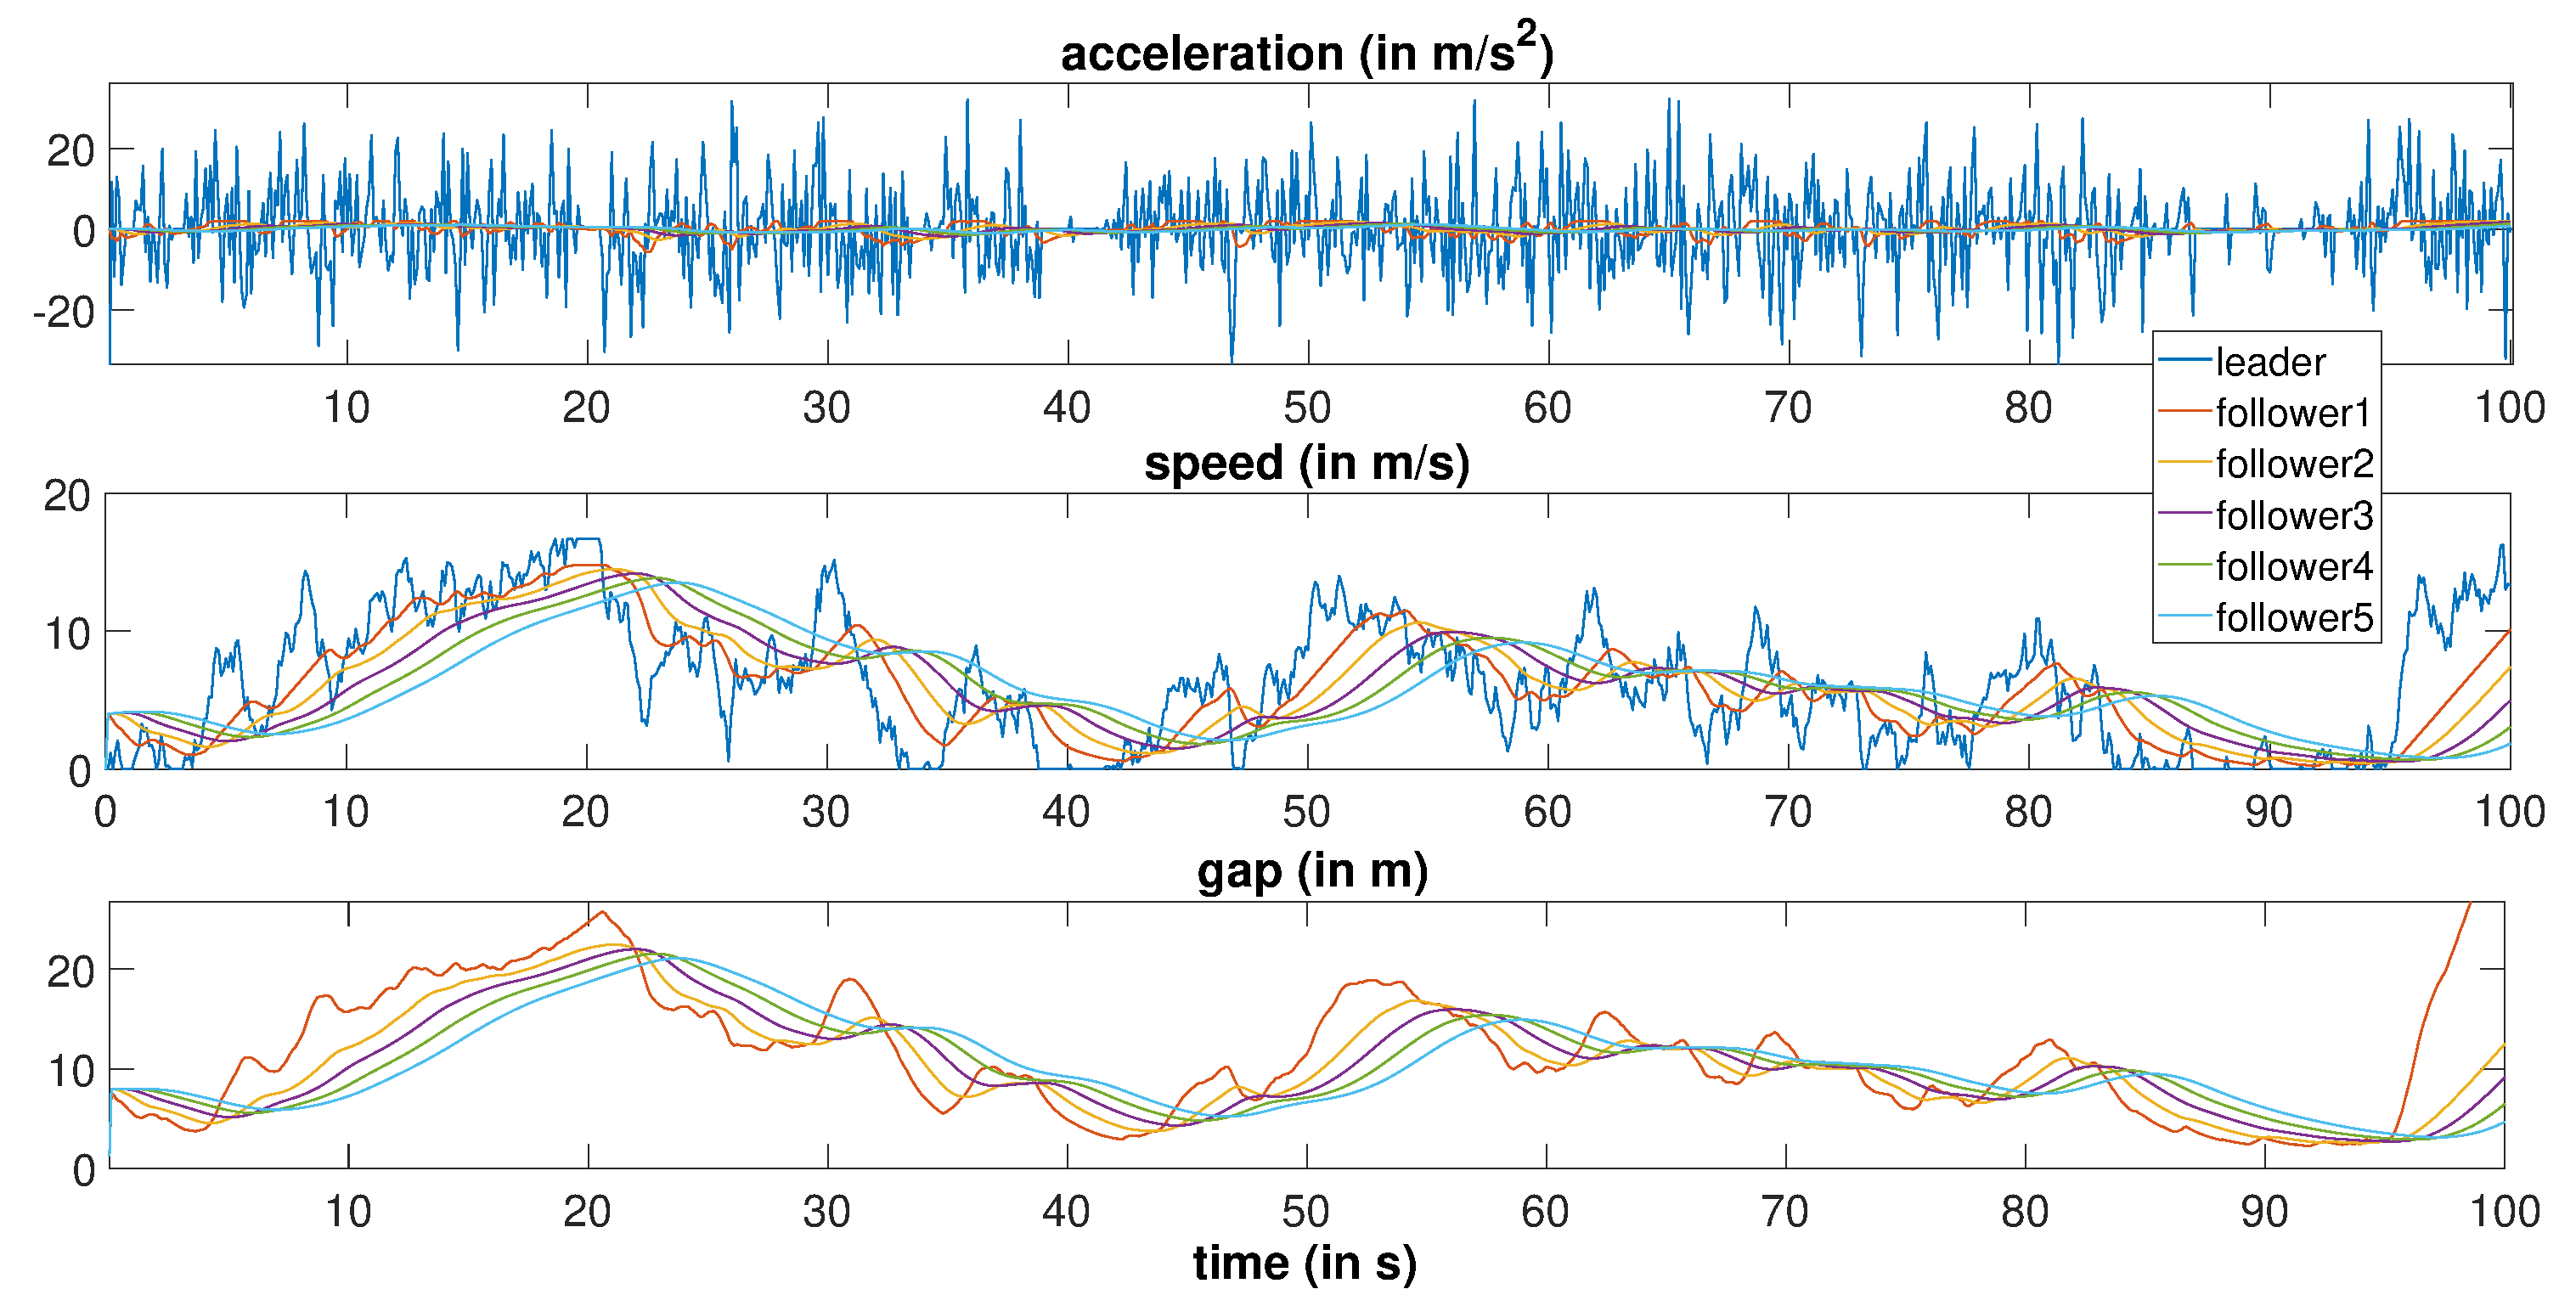
\includegraphics[width=0.95\textwidth]{images/AR1Kolonne}
	\caption{Response to a leader trajectory based on a AR(1) process}
	\label{fig:AR1Kolonne}
\end{figure}


\subsection{Response to a real leader trajectory}

In a further scenario, the abilities of the RL strategy are evaluated
with a real leader trajectory (Fig.~\ref{fig:PunzoKolonne})
\martinc{Die Tilde im Latex Quelltext bedeutet ein reserviertes
  Leerzeichen, bei dem kein Zeilenumbruch stattfinden darf}. This
trajectory comes from \martin{platoon driving} experiments in Napoli
where \martin{high-precision distance data between the platoon
vehicles} were obtained (reference to Punzo et al.). \martinc{wdh
  gestrichen} Similar to the experiment from
Section~\ref{sec:stringStability}, string stability and the reduction
of  the acceleration variance, shown by the red bars in Figure
\ref{fig:VarAccComp}, is demonstrated. At time $t = 140s$ the leader
stands still, and it can be observed, that all following vehicles are
keeping the minimum distance $s\sub{min}$ to the leader.  


\begin{figure}
	\centering
	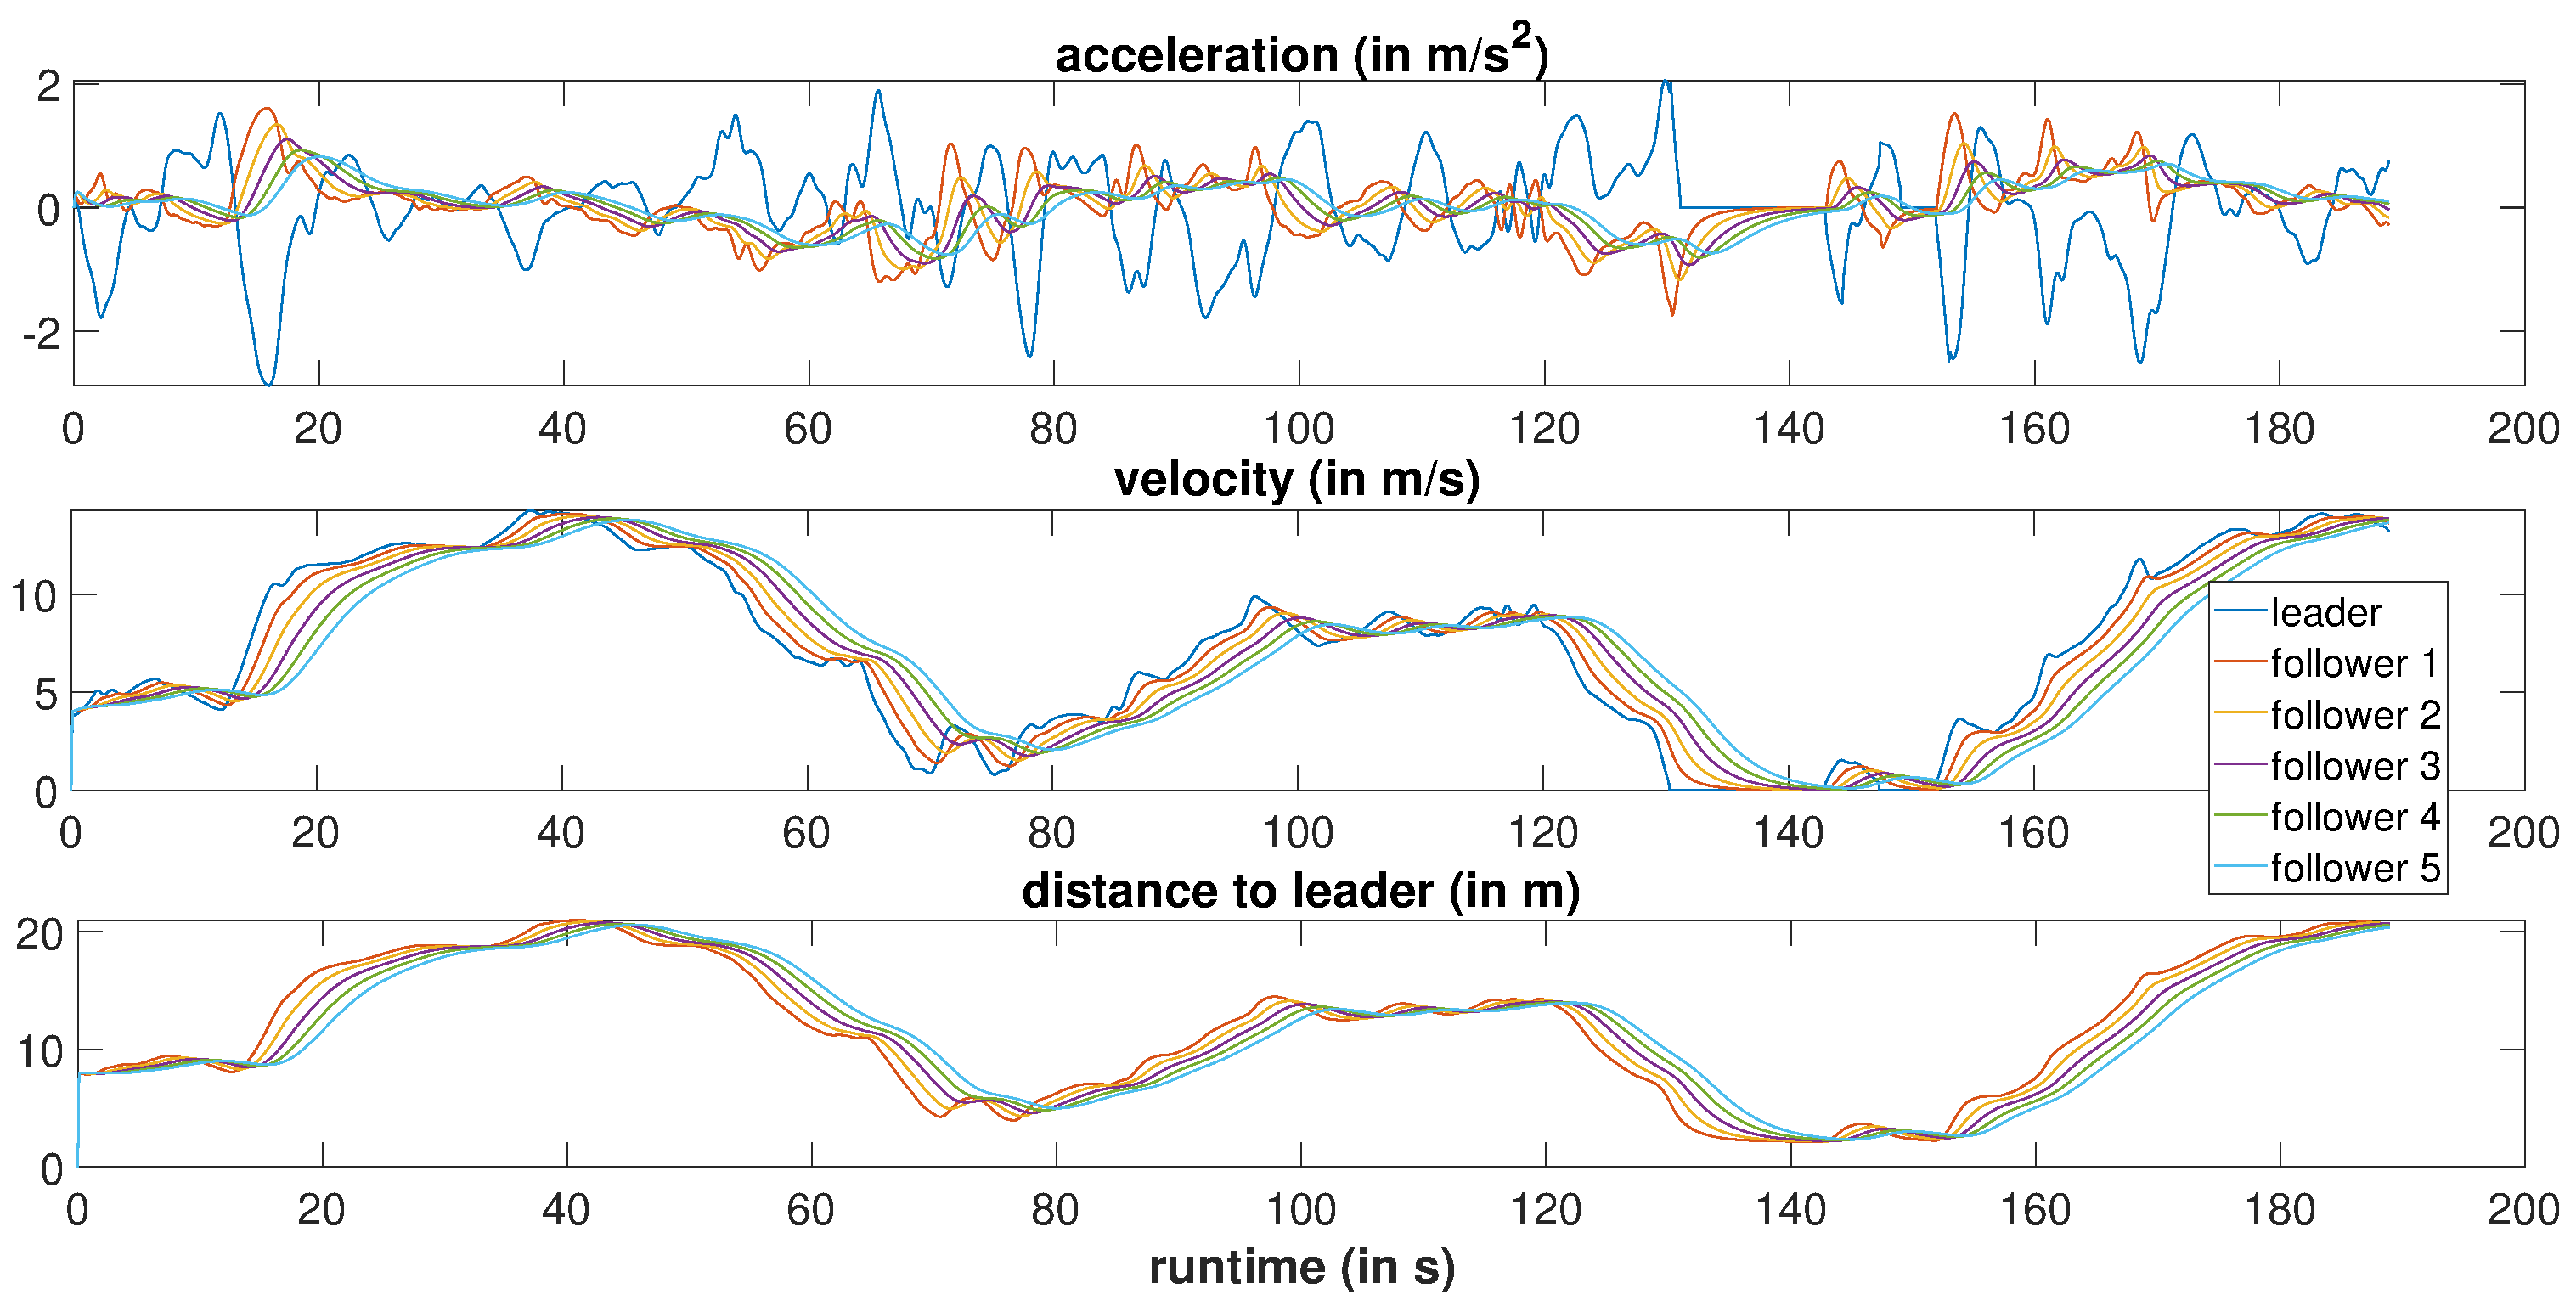
\includegraphics[width=0.95\textwidth]{images/PunzoKolonne}
	\caption{Response to a real leader trajectory \martinc{Die
            leader acceleration hat das falsche Vorzeichen bzw passt
            f\"ur $t>\unit[160]{s}$ \"uberhaupt nicht! Gilt auch f\"ur
        die n\"achste Abbildung}}
	\label{fig:PunzoKolonne}
\end{figure}


\subsection{Response of different driver characteristics}
\label{sec:differentT}

As mentioned in Section \ref{rewardFunction}, different driving styles
can be achieved by adjusting the parameters of the reward
function. Three RL agents has been trained on a reward function, that
differs in the desired time gap $T$ das between following and
leading vehicle ($T_{1} = 1.0s$, $T_{2} = 1.5s$, $T_{3} =
2.0s$). Figure \ref{fig:differentT} shows the result of these agents,
following the real leader trajectory from Napoli. It can be observed,
that a lower value for $T$ results in closer driving to the
leader \martin{which can be considered as a more ``aggressive''
  driving style. Since this also means that there are less options in
increasing driving comfort without affecting safety, the follower's
accelerations and decelerations also increase although the relatve
weighting $w_2/w_3$ of the safety and comfort aspects in Eq.~\eqref{rt} has not been
changed.} 

\begin{figure}
	\centering
	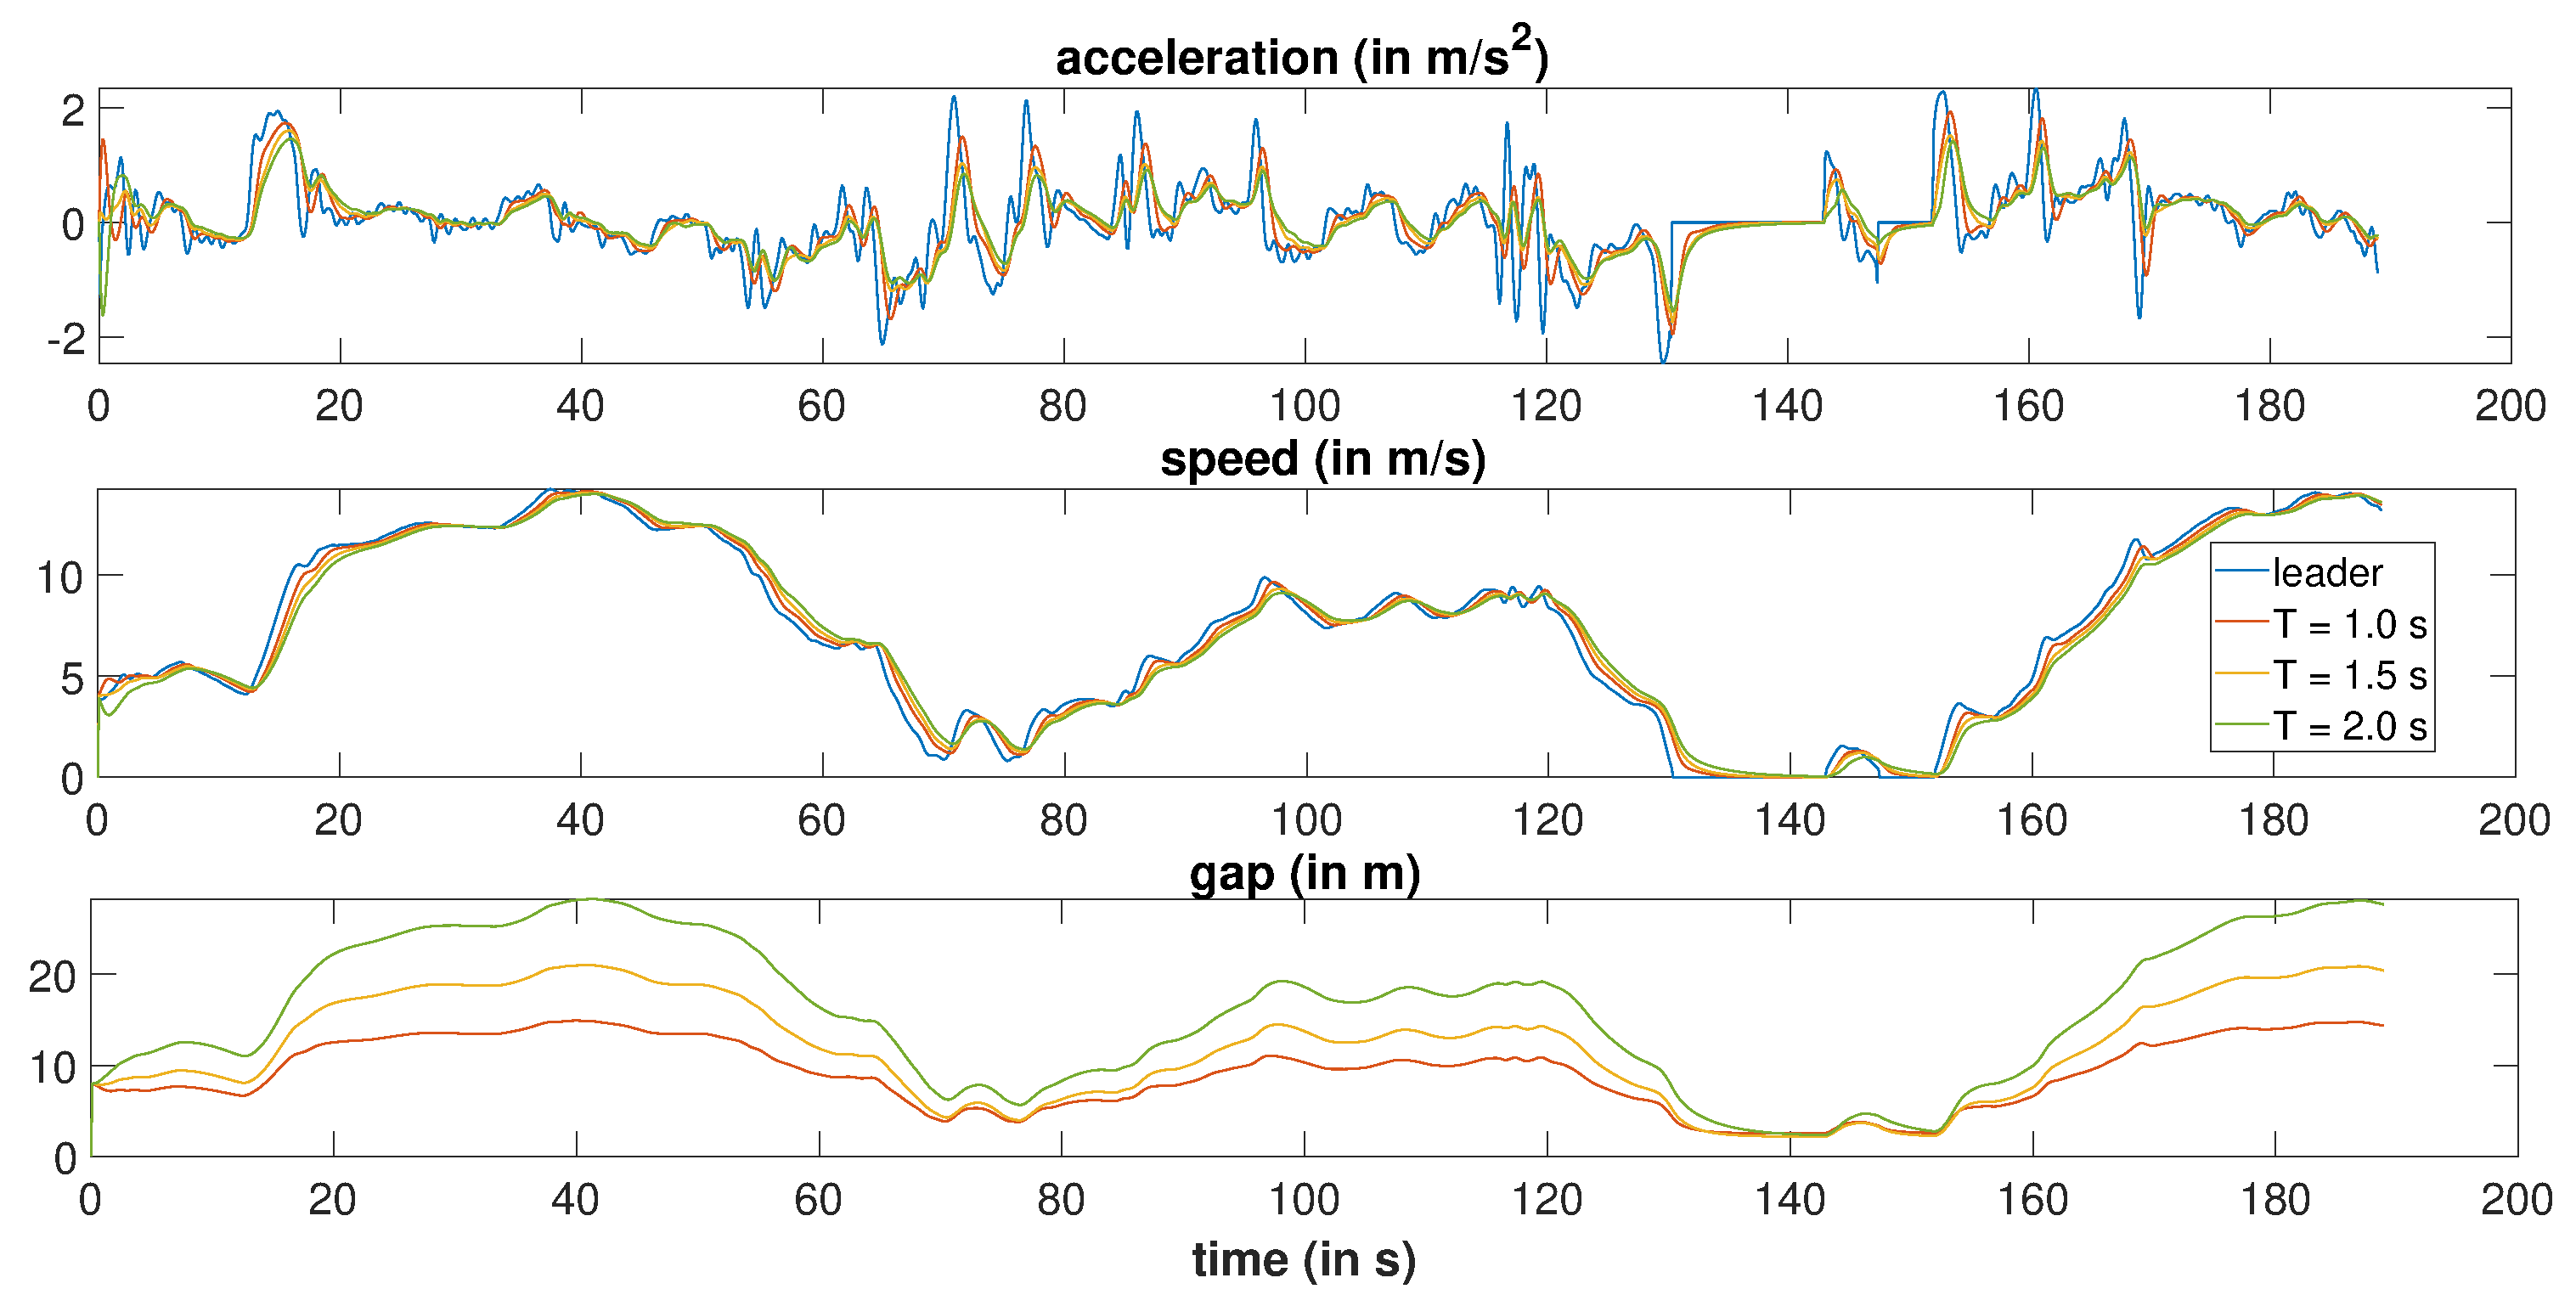
\includegraphics[width=0.95\textwidth]{images/differentT}
	\caption{Impact of different\martin{ly} parametrized RL agents
          on the driving behavior \martinc{Fehler Leader-Beschl., vgl. vorherige Abb.}}
	\label{fig:differentT}
\end{figure}


\subsection{Cross validation with the Intelligent Driver Model}
\martinc{reformulated}
To compare the performance of the RL agent with that of
classical car-following models, we chose the commonly used
Intelligent-Driver Model (IDM)\cite{Opus} whose acceleration is given
by
\begin{equation}
\label{eq:IDM}
a=a\sub{max}\left(1-\left(\frac{v}{v\sub{des}}\right)^{4}-\left(\frac{s^{*}\left(v, \Delta v\right)}{s}\right)^{2}\right),
\end{equation}
with
\begin{equation}
\label{eq:IDMsstar}
s^{*}\left(v, \Delta v\right)=s\sub{min}+\max \left(0,vT+\frac{v \Delta v(v-v_l)}{2 \sqrt{a\sub{max} b\sub{comf}}}\right).
\end{equation}
Notice that the IDM parameters desired
speed $v\sub{des}$, minimum gap $s\sub{min}$, time gap $T$, maximum
acceleration $a\sub{max}$, and
comfortable deceleration $b\sub{comf}$ are a subset of that of the RL reward
function. 

First, we calibrate the IDM on the Napoli data set by
minimizing the sum of squares of the relative gap error,
$\mathrm{SSE}(\ln s)$, of the first follower with respect to the
data (cf. Table~\ref{tab:IDMparameters}). The same parameters are also
assumed for the reward function of the RL agent before it was trained
on the artificial AR(1) generated leader speed profile
\martinc{check!}. Notice that the RL agent used the Napoli data only
indirectly by parameterizing its reward function.
\begin{table}
	\caption{\martin{IDM parameters calibrated to the Napoli
            data and also used for the reward function of the RL agent}} 
	\label{tab:IDMparameters} 
	\begin{center}
		\begin{tabular}{ p{0.14\textwidth} |p{0.1\textwidth}  } 
		Parameter & Value   \\ \hline
			$T$ & $0.83s$\\
			$s\sub{min}$ & $4.90m$\\
			$a\sub{max}$ & $4.32m/s^2$\\
			$b\sub{comf}$ & $2.34 m/s^2$\\
			$v\sub{des}$ & $33.73m/s$
			
		\end{tabular}
	\end{center}
\end{table}

Figure \ref{fig:IDMvsRL} shows the results for: First, the RL agent, calibrated on the real follower data. Second, the IDM, calibrated on the follower data. And third, the real follower of the Napoli experiment. To evaluate the performance, for both approaches the respective objective function has been computed. The objective function of the RL agent correspondences to the reward function, while the Goodness-of-Fit Function $SSE(s)$ defines the objective function of the IDM. A comparison between RL agent and IDM for both, the reward function and the Goodness-of-Fit Function, is shown in Table \ref{tab:objectiveFunc}. For both objectives the RL agent shows a better performance.

\begin{figure}
	
	\centering
	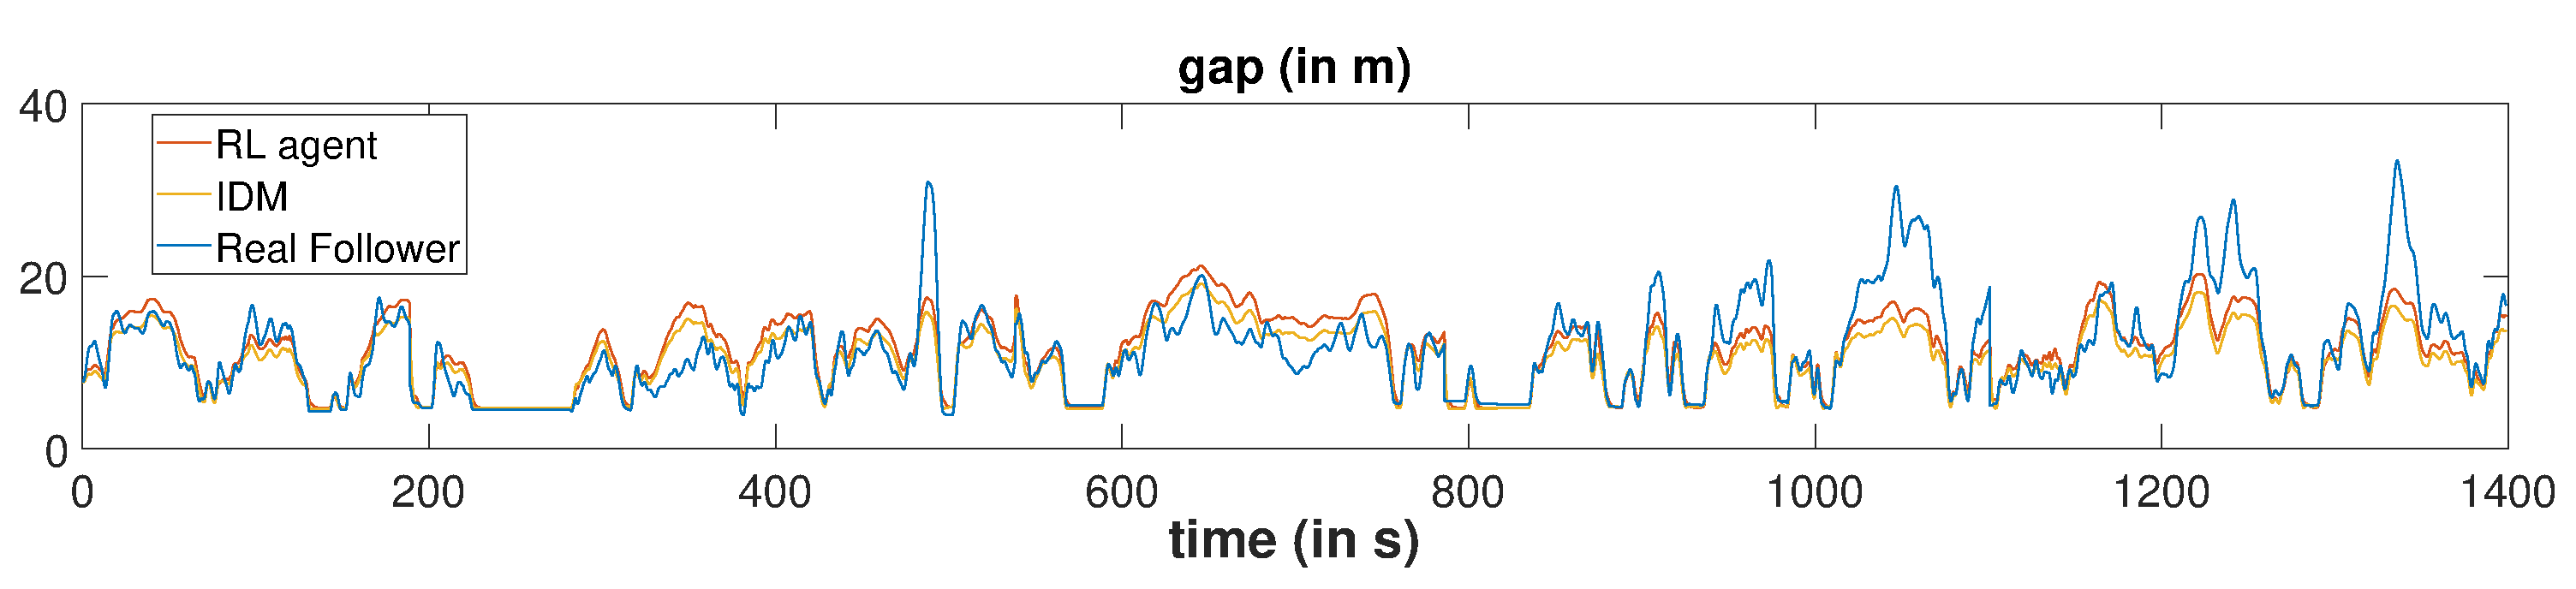
\includegraphics[width=0.95\textwidth]{images/IDMvsRL_dist}
	\caption{Comparison between IDM and RL agent, calibrated on the same set of parameters}
	\label{fig:IDMvsRL}
\end{figure}

\begin{table}
	\caption{Comparison between calibrated RL agent and IDM for accumulated Reward and Goodness-of-Fit Function $SSE(log(s))$} 
	\label{tab:objectiveFunc} 
	\begin{center}
		\begin{tabular}{p{0.3\textwidth} | p{0.2\textwidth} p{0.2\textwidth}  } 
			& RL agent & IDM   \\ \hline
			$SSE(log(s))$ & $389.10$ &  $418.05$	\\
			Accumulated Reward &  $8.23 \times 10^3$   & $8.08\times 10^3$
			
		\end{tabular}
	\end{center}
\end{table}


\section{Conclusion/Discussion}
evaluation of safety and comfort, comparison to IDM



\bibliography{RL_vehicles_references}

\end{document}
